
\chapter{Implementation: LSP server architecture}
\label{lspimplementation}

CCDetect-LSP is integrated into IDEs via the Language server protocol. The tool starts up as
an LSP server, which an IDE client can connect to and send/receive messages from. The goal
of the LSP server/client interaction is to give users of the tool an overview of all
clones as they appear. The LSP server is implemented in Java with the LSP4J library which
provides an abstraction layer on top of the protocol which is easier to work with
programmatically.

The LSP server shows error-messages (diagnostics) which indicate which section of code a
clone covers, they also provide information about the matching clones and code-actions to
navigate between them. Whenever source code is edited, the LSP server receives a message
containing information about what has changed. The LSP server then generates a new list of
clones, and displays those to the client instead.

The following user-stories shows how interaction with the LSP server works.

\begin{itemize}
	\item A programmer wants to see code clones for a file in their project, the
	      programmer opens the file in their IDE and is displayed diagnostics in the code
	      wherever there are detected clones. The matching code clones are not necessarily
	      in the same file.

	\item A programmer wants to see all code clones for the current project. The
	      programmer opens the IDEs diagnostic view and will see all code clones detected
	      as diagnostics there. The diagnostic will contain information like where the clone
	      exists, and where the matching clone(s) are.

	\item A programmer wants to jump to one of the matches of a code clone in their
	      editor. The programmer moves their cursor to the diagnostic and will see a list of
	      the matching code clones. The programmer will select the wanted code clone which
	      will move the cursor to the file and location of the selected code clone.
          Alternatively, a code-action can be invoked to navigate, if the client does not
          implement the \verb|DiagnosticRelatedInformation| interface.

      \item A programmer wants to remove a set of clones by applying the
          ``extract-method'' refactoring. The programmer performs the necessary
          refactorings, and will see that all the previously detected clones are gone when
          the LSP server updates.

\end{itemize}

\begin{figure}
	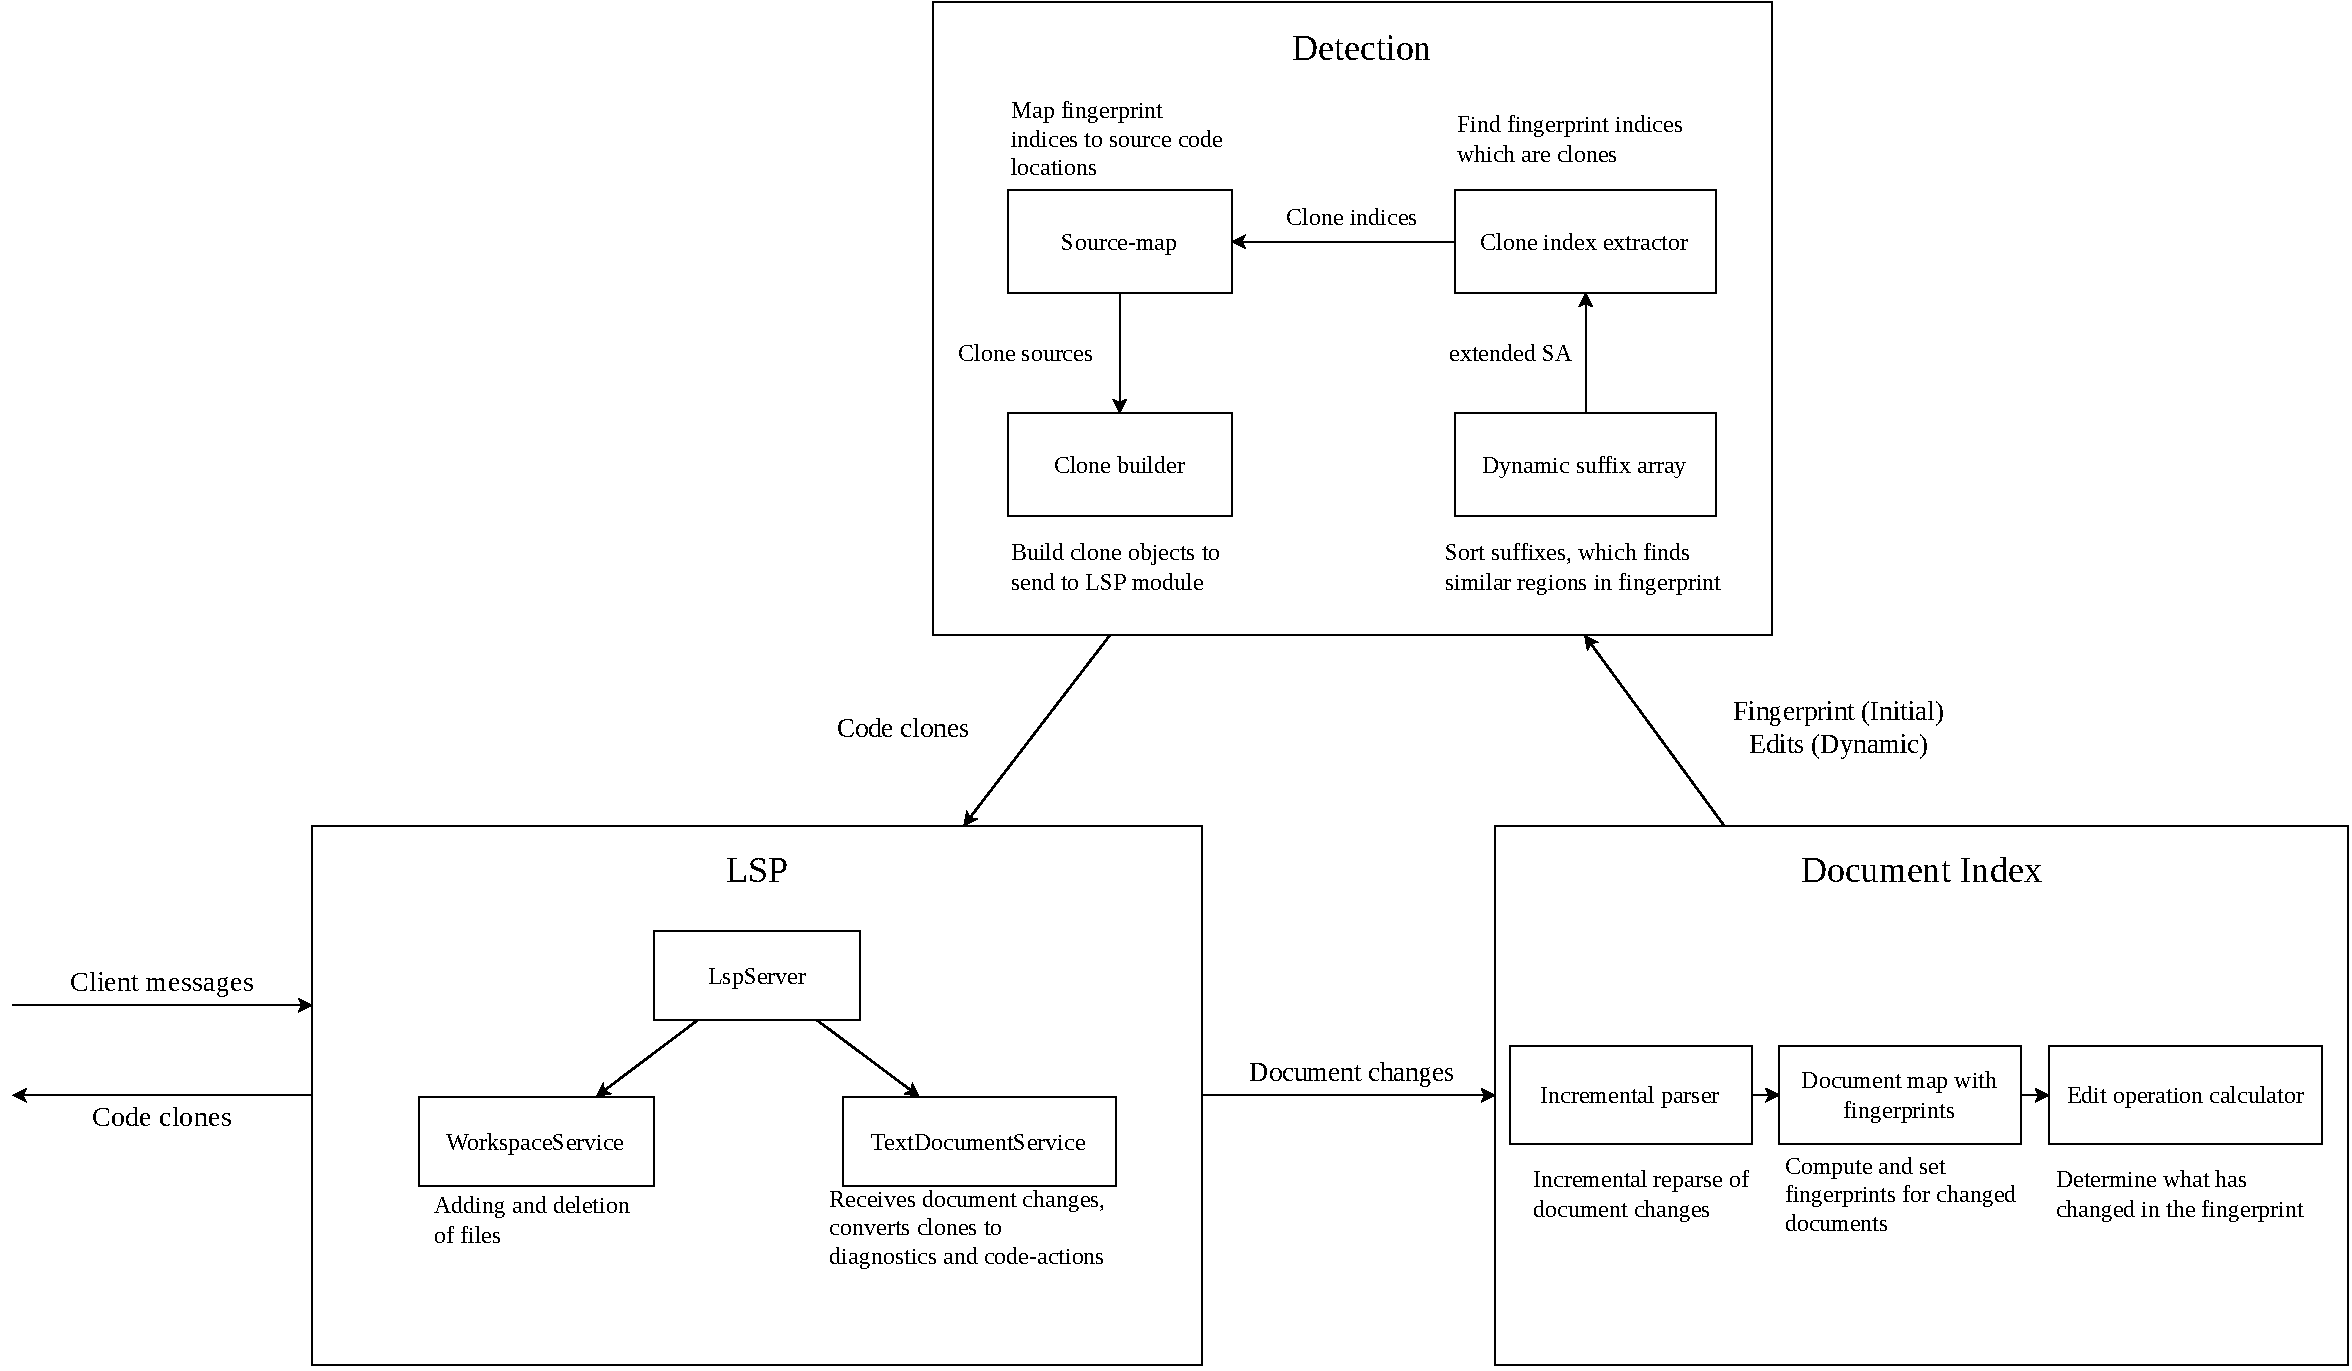
\includegraphics[width=\textwidth]{figures/architecture.drawio.pdf}
	\caption{Tool architecture}
	\label{fig:architecture}
\end{figure}

Figure \ref{fig:architecture} shows the architecture of the tool. The LSP module
communicates with the IDE and delegates the work of handling documents to the document
index. Detection of clones is delegated to the detection module. The LSP module receives a
list of clones from the detection module which is then converted to LSP diagnostics and
code-actions which is finally sent to the client.

\section{Document index}

Upon starting, the LSP server requires indexing of the project for conducting analysis.
This involves creating an index and inserting all the relevant documents in the code base.
A document contains the content of a file along with extra information such as the file's
URI and some information which is useful for the later clone detection. We define the
following interface for our documents:

\begin{lstlisting}
    interface Document {
        String uri,
        String content,
        AST ast,

        // Location in fingerprint
        int start,
        int end

        // Used for incremental updates
        int[] fingerprint,
        boolean open,
        boolean changed,
    }
\end{lstlisting}

Each document in the index primarily consists of the contents, the URI and the AST of the
document in its current state. Storing the AST will be useful for the incremental
detection algorithm.

There are two things to consider when determining which files should be inserted into the
index. First, we are considering only files of a specific file type, since the tool does
not allow analysis of multiple programming languages at the same time. Therefore, the
index should contain for example only \verb|*.java| files if Java is the language to
analyze. Secondly, all files of that file type might not be relevant to consider in the
analysis. This could for example be generated code, which generally contains a lot of
duplication, but is not practical or necessary to consider as duplicate code, since this
is not code which the programmer interact with directly. Therefore, the default behavior
is to consider only files of the correct file type, which are checked into Git. The tool
supports adding all files in a folder, or all files checked into Git.

When a document is first indexed by the server, the file contents is read from the disk.
However, as soon as the programmer opens this file in their IDE, the source of truth for
the files content is no longer on the disk, as the programmer is changing the file
continuously before writing to the disk. The LSP protocol defines multiple RPC
messages which the client sends to the server in order for the server to keep track of
which files are opened, and the state of the content of opened files.

Upon opening a file, the client will send a \verb|textDocument/didOpen| message to the
server, which contains the URI for the opened file. The index will at this point set the
flag \verb|open| for the relevant document and stops reading its contents from disk.
Instead, updates to the file are obtained via the \verb|textDocument/didChange| message.
This message can provide either the entire content of the file each time the file changes,
or it can provide only the changes and the location of the change. Receiving only the
changes will be useful for this algorithm when the analysis incrementally reparses the
document.

\section{Displaying and interacting with clones}

When detection is finished and the list of clones is ready, the LSP module will convert
clones into diagnostics and code-actions which can be interacted with from the client. For
diagnostics, each clone object is converted into a diagnostic which has a range and some
information about the clone. The diagnostic displays an error in the client which also has
information for each matching clone. This is achieved this by attaching
\verb|DiagnosticRelatedInformation| to a diagnostic which is defined in the protocol. When
all the code clones have been converted to diagnostics, the server sends a
\verb|textDocument/publishDiagnostics| which sends all the diagnostics in JSON-RPC format.
For code-actions, the process is similar, for each clone pair, we create a code-action
which navigates from one to the other, using the \verb|window/showDocument| message. These
code-actions are similarly sent to the client via the \verb|textDocument/codeAction|
message, but this message is only invoked when the client specifically requests code
actions at a certain location.

Figure \ref{fig:vscodeclones} shows how clones are displayed in the VSCode IDE. Code
clones are displayed inline in the file as an ``Information'' diagnostic, and when hovered
over, the client shows the \verb|DiagnosticRelatedInformation| information of the diagnostic
where all the matching clones are displayed and can be clicked to navigate to the
corresponding match. For a client which may not implement the
\verb|DiagnosticRelatedInformation| message (which was added in LSP version 3.16), invoking
the code-action to navigate to the matching clone is another option.

\begin{figure}
	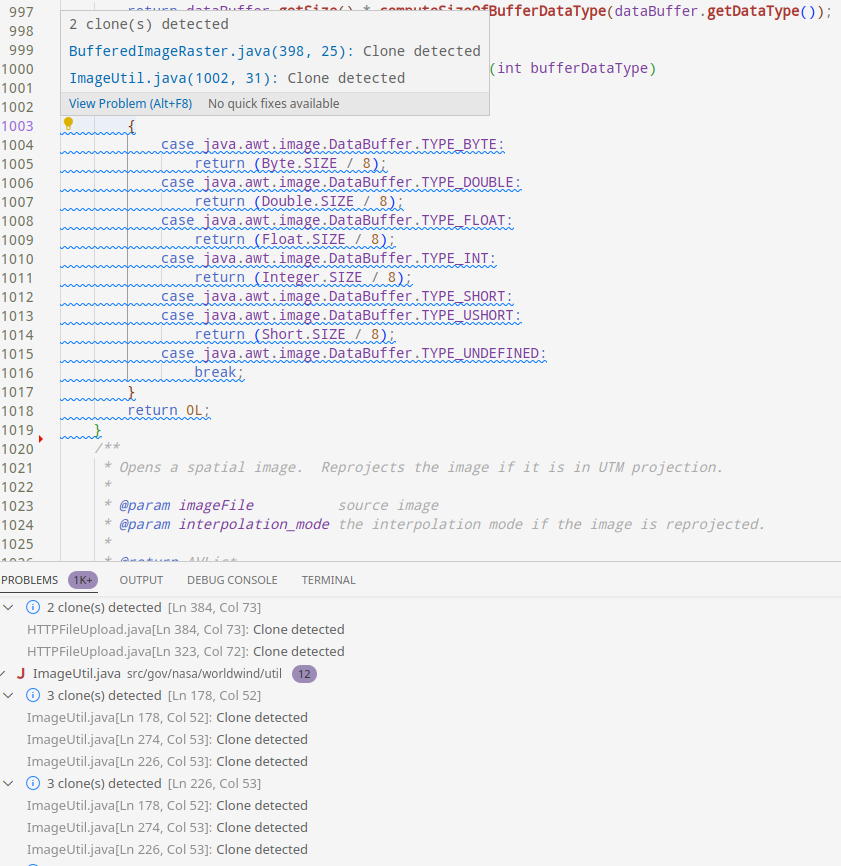
\includegraphics[width=\textwidth]{figures/vscodecodeclone.png}
	\caption{Code clones displayed in the VSCode IDE}
	\label{fig:vscodeclones}
\end{figure}

\chapter{Implementation: Initial detection}


This chapter discusses the detection module of CCDetect-LSP. It consists of the detection
algorithm which takes the document index as input, and outputs a list of code clones. The
initial input to the algorithm will be the raw source code of each document in the index,
in text format.

The algorithm detects syntactical type-1 code clones, based on a token-threshold. Clones
detected are therefore snippets of source-code which has at least $N$ equal tokens, where
$N$ is a configurable parameter. There are also two types of clones which are filtered:

\begin{itemize}
    \item Clones which are completely contained within another larger clone are filtered.
    \item Clones cannot extend past the end of a fragment.
\end{itemize}


In broad strokes, the algorithm first selects the relevant parts of source code to detect
code clones in (fragment selection), then transforms the selected fragments into a smaller
representation (fingerprinting). For the matching, an extended suffix array for the fingerprint
is constructed, where the LCP array is used to find long matching instances of source code.
Finally, clones are filtered and aggregated into clone classes before they are
source-mapped back to the original source-code locations, which the LSP server can display
as diagnostics.

\section{Fragment selection}

The first phase of the algorithm involves extracting the relevant fragments of source code
which should be considered for detection. A fragment in this case is considered as a
section of abstract syntax, meaning that a particular type of node in the AST and the
tokens it encompasses should be extracted. Since the algorithm is language agnostic, it is
not feasible to have a single algorithm for fragment extraction or to define a separate
fragment extraction algorithm for every possible language. Therefore, a parser generator
tool is used, which can generate the code for parsing any programming language given a
grammar. We use Tree-sitter, a parser generator with incremental parsing and
error-recovery capabilities, as well as a query language for finding any type of node in
the AST~\cite{treesitter}. Tree-sitter queries are flexible queries to extract specific
nodes or subtrees. For example, in Java it would be natural to consider only methods. The
Tree-sitter query for selecting only the method nodes in a Java programs AST would be:

\begin{equation}
    (\mathrm{method\_declaration\ } \text{@method})
\end{equation}

This Tree-sitter query selects the node with type \verb|method_declaration| and
``captures'' it with the \verb|@method| name, so that it can be further processed by the
program. Readers interested in the details of the query system are referred to the
Tree-sitter documentation~\cite{treesitter}.

Using a tree-sitter query, the algorithm parses the program into an AST, queries the tree
for all the nodes which matches the query (taking care not to capture nodes which are
children of already captured nodes) and extracts all the tokens which the node covers.

\Todo{Algorithm?}

Implementing something similar for another parser/AST could be as simple as traversing
the tree until a node of a specific type is found, using the visitor pattern~\cite[366]{GangOfFour}.


\section{Fingerprinting}

\Todo{Høyere abstraksjonsnivå med infinite alphabets}

\newsavebox{\firstlisting}
\begin{lrbox}{\firstlisting}
\begin{lstlisting}
public class Math() {
    public int multiplyByTwo(int param) {
        return param * 2;
    }

    public int addTwo(int param) {
        return param + 2;
    }
}
\end{lstlisting}
\end{lrbox}
\begin{figure}[htp]
	\begin{center}
        \subfloat[Source-code] {
            \usebox{\firstlisting}
        }
        \hspace{1cm}
        \subfloat[Fingerprint mapping] {
            \begin{tabular}{l | l}
                Token & Fingerprint \\
			    \hline
                public & 2 \\
                int & 3 \\
                multiplyByTwo & 4 \\
                ( & 5 \\
                param & 6 \\
                ) & 7 \\
                \{ & 8 \\
                return & 9 \\
                * & 10 \\
                2 & 11 \\
                ; & 12 \\
                \} & 13 \\
                addTwo & 14 \\
                + & 15 \\
            \end{tabular}
        }

        \vspace{0.5cm}
        \subfloat[Fingerprint, terminals underlined] {
            [ 2, 3, 4, 5, 3, 6, 7, 8, 9, 6, 10, 11, \underline{1}, 2, 3, 14, 5, 3, 6, 7,
            8, 9, 6, 15, 11, \underline{1}, \underline{0} ]
        }
	\end{center}
	\caption{Example fingerprint of Java source-code}
	\label{fig:fingerprint}
\end{figure}

The next phase of the algorithm is to transform the extracted source code into a
representation which is less computationally heavy for the matching algorithm. The goal is
to reduce the total size of the input which needs to be processed by the matching
algorithm.

Since the algorithm that is used for matching is based on a suffix array, the
representation should be in a format similar to a string, which is the standard input to a
suffix array construction algorithm. However, it is not strictly necessary to use strings.
The essential property of the input array is that we have an infinite alphabet where each
element is comparable. Therefore, we can use an array of integers instead, which is
preferable, since there are often a lot more unique integers available than unique
characters in a programming language. The algorithm will need to have a lot of unique
elements in the representation because each unique token value will be represented by
a single unique element of the alphabet, therefore integers are a good choice.


The algorithm utilizes fingerprinting in order to reduce the size of the representation.
Fingerprinting is a technique which involves taking some part of the input and mapping it
to a smaller bit string, which uniquely identifiers that part. In this case, the algorithm
takes each token of the source-code, and maps it to an integers bit string. Each unique
token value (tokenized by tree-sitter) is mapped to unique integer values. Note that the
algorithm maps token values, not types. This ensures that tokens of different
variable-names and literals are not seen as equal. Figure \ref{fig:fingerprint} shows how
a sample Java program could theoretically be fingerprinted. The fingerprint mapping starts
its ``count'' at 2 to make space for some terminating characters. Each fragment is
terminated by a $1$ and the fingerprint is ultimately terminated by a $0$. Having these
values in the fingerprint will be useful for the matching algorithm where the suffix array
is constructed and utilized for detection. The fingerprint of each fragment is stored in
the relevant document object.


\section{Suffix array construction}


The next step is to input the fingerprint into a suffix array construction algorithm
(SACA), so that the suffix array can be used to find maximal repeats. Recall that we
discussed the suffix array in \cref{prelimalgos} and that the suffix array of a string
sorts all the suffixes of the string, making it simple to find similar regions of text,
since similar suffixes will be next to each other in the suffix array. All the
fingerprints which are stored in each document object will now be concatenated to be
stored in a single integer array (with terminators after each fragment), which the suffix
array (SA), inverse suffix array (ISA) and longest-common prefix array (LCP) is computed
from.

We have utilized a straight-forward implementation of the ``Induced sorting
variable-length LMS-substrings'' algorithm~\cite{LinearTimeSuffixArraySAIS} which computes
a suffix array in linear time. The following section will give high-level overview of how
the algorithm works. 

The algorithm will be assumed to have a string as its input, as this is most common for
suffix arrays, and working with strings can be more clear to the reader when considering
suffixes. The algorithm is still applicable to our fingerprint, since an array of integers
will work similarly to a string when given as input.

The ``Induced sorting variable-length LMS-substrings'' algorithm (often abbreviated SA-IS)
is an algorithm that works by divide and conquering the suffix array and inducing how to
sort the suffixes of the string $S$ from a smaller string, $S_1$. $S_1$ consists of the
``building blocks'' of $S$ and will make it simple to compute the rest of the suffix array
of $S$. First, we will introduce some definitions and theorems used for the algorithm.
Input to the algorithm is a string $S$ with length $n$. Let $\mathrm{suffix}(S, i)$ be the
suffix in S starting at position i.

\begin{definition}[L-type and S-type suffixes] A suffix starting at position $i$ in a
    string $S$ is considered to be L-type if it is lexicographically larger than the next
    suffix at position $i + 1$. Meaning that $\mathrm{suffix}(S, i) > \mathrm{suffix}(S,
    i+1)$. Conversely, a suffix is considered to be S-type if $\mathrm{suffix}(S, i) <
    \mathrm{suffix}(S, i+1)$. The sentinel suffix (\$) of $S$ is always S-type.
\end{definition}

\begin{algorithm}[htp]
  \SetAlgoLined\DontPrintSemicolon
    \algo{\SuffixTypes{S}}{
        $\Var{n} \gets \Access{\Var{S}}{len}$ \;
        $\Var{Stype} \gets \True$ \;
        $\Var{Ltype} \gets \False$ \;\;

        $\Var{types} \gets \mathrm{Bitset\ of\ size\ n}$ \;\;

        $\Set{$\Var{types}, \Var{n}, \Var{Stype}$}$ \;
        $\Set{$\Var{types}, \Var{n} - 1, \Var{Ltype}$}$ \;\;

        \For{$i \From n - 2 \To 0$}{

            \uIf{$\Access{\Var{S}}{\Var{i}} <  \Access{\Var{S}}{\Var{i} + 1}$}{
                $\Set{$\Var{types}, \Var{i}, \Var{Stype}$}$
            }
            \uElseIf{$\Access{\Var{S}}{\Var{i}} >  \Access{\Var{S}}{\Var{i} + 1}$}{
                $\Set{$\Var{types}, \Var{i}, \Var{Ltype}$}$
            }
            \Else{
                $\Set{$\Var{types}, \Var{i}, \Get{$\Var{types}, \Var{i} + 1$}$}$

            }
        }

        \Return $\Var{types}$
    }

  \vspace{0.5cm}
  \caption{Compute suffix types of a string}
  \label{alg:suffixtypes}
\end{algorithm}


\begin{table}
    \begin{center}
        \begin{tabular}[c]{l l l l l l l}
            B & A & N & A & N & A & \$ \\ 
            L & \underline{S} & L & \underline{S} & L & L & \underline{S} \\ 
            0 & 1 & 2 & 3 & 4 & 5 & 6 \\ 
        \end{tabular}
    \end{center}
    \caption{Suffix types of S = BANANA\$, LMS characters underlined}
    \label{tab:suffixtypesbanana}
\end{table}


\begin{table}
    \begin{center}
        \begin{tabular}[c]{r|cccc}
            Buckets & \$ & A & B & N\\
            Initial & \{ -1 \} & \{ -1, -1, -1 \} & \{ -1 \} & \{ -1, -1 \}\\
            Slot LMS & \{  6 \} & \{ -1,  3,  1 \} & \{ -1 \} & \{ -1, -1 \}\\
            Slot L-type & \{  6 \} & \{  5,  3,  1 \} & \{  0 \} & \{  4,  2 \}\\
            Slot S-type & \{  6 \} & \{  5,  3,  1 \} & \{  0 \} & \{  4,  2 \}\\
        \end{tabular}

        \vspace{0.5cm}
        \begin{tabular}[c]{r|c|c}
                    & \$ & 0 \\
            Mapping & ANA\$ & 1 \\
                    & ANA & 2 \\
        \end{tabular}

        \vspace{0.5cm}

        \begin{tabular}[c]{l|c}
                    $S_1$ & $210$ \\
                    SA of $S_1$ & $[2, 1, 0]$ \\
                    Sorted LMS-substrings & $[6, 3, 1]$ \\
        \end{tabular}

    \end{center}
    \caption{Building $S_1$ and sorting LMS-substrings of S = BANANA\$}
    \label{tab:bucketinglms}
\end{table}


Note that two suffixes in the same string cannot be lexicographically equal, therefore all
cases are handled by this definition. Determining the type of each suffix can be done in
$O(n)$ time by scanning $S$ from right-to-left and observing the following properties:
$\mathrm{suffix}(S, i)$ is L-type if $\Access{S}{i} > \Access{S}{i + 1}$. Similarly,
$\mathrm{suffix}(S, i)$ is S-type if $\Access{S}{i} < \Access{S}{i + 1}$. If
$\Access{S}{i} = \Access{S}{i + 1}$, then $\mathrm{suffix}(S, i)$ is the same value as
$\mathrm{suffix}(S, i + 1)$. This is true because if the first character of the current
suffix is not equal to first character of the next suffix, we already know the type based
on the first character. If the first character is equal however, we have effectively
transformed the problem to finding the type of the next suffix, since we are now comparing
the second character of the current suffix, with the second character of the second
suffix. Since we have already computed the type of the next suffix, we can reuse the value.
Figure \ref{alg:suffixtypes} shows an algorithm which determines the type of each suffix
in a string in $O(n)$ time and \ref{tab:suffixtypesbanana} shows an example.

\begin{definition}[LMS character]

    An LMS (Left-most S-type) character in a string $S$ is a position $i$ in $S$ such that
    $S[i]$ is S-type and $S[i-1]$ is L-type. An LMS-suffix is a suffix in $S$ which begins
    with an LMS character. The final character of $S$ (the sentinel) is always an LMS
    character and the first character is never an LMS character.

\end{definition}

\begin{definition}[LMS-substring]

    An LMS-substring in a string $S$ is a substring $S[i..j]$ in $S$ such that $i \neq j$,
    $S[i]$ and $[j]$ are LMS characters and there are no other LMS characters between. The
    sentinel character is also an LMS-substring and is the only LMS-substring of length
    $\leq 3$

\end{definition}

LMS-substrings form "basic-blocks" in the string $S$. Each LMS-substring is mostly
lexicographically decreasing or increasing, which is easier to sort. Table
\ref{tab:bucketinglms} shows that in the string BANANA\$ there are 3 S-type suffixes
and all of them form LMS-substrings (AN, ANA, \$). Using this notion, we can sort all
suffixes recursively using the following theorems:

\begin{theorem}

    Given sorted LMS-suffixes of $S$, the rest of the suffix array can be induced in linear
    time. 

\end{theorem}

\begin{theorem}
    There are at most $n / 2$ LMS-substrings in a string $S$ of length n.
\end{theorem}

We can construct a smaller string $S_1$ by first sorting the LMS-substrings. Sorting
LMS-substrings can be done by first bucket-sorting each LMS-substring by its first
character. The buckets are represented by arrays and each LMS-substring is inserted at the
end of the correct bucket. Afterwards, L-type suffixes are bucketed by iterating over the
buckets, and for each suffix in the bucket, insert the suffix to the left, if it is
L-type. Meaning that if we encounter the suffix at position 6, the suffix at position 5 is
bucketed if it is L-type. Finally, S-type suffixes are bucketed similarly in the same
fashion, but the buckets are scanned from right-to-left and suffixes are inserted at the
end of the bucket. This final step could possibly change the ordering of the
LMS-substrings.

After sorting, each equal LMS-substring is given a unique increasing integer value. Two
LMS-substrings are considered equal if they are equal in terms of length, characters and
types. $S_1$ is now built by mapping each LMS-substring to its unique value, and
concatenating them in the original ordering. $S_1$ is now a smaller case which is used in
the recursion. The string is at most $n / 2$ in size, meaning there will be at most
$\log_2(n)$ recursive calls. The recursive call will return the suffix array of the $S_1$.
Nong et al. proves a theorem which shows that sorting $S_1$ is
equivalent to sorting the LMS suffixes of $S$. Therefore, the suffix array of $S_1$ can be
mapped to the LMS suffixes of $S$~\cite{LinearTimeSuffixArraySAIS}.

The base-case of the recursion is when the suffix array can be computed simply by
bucketing each suffix, which happens when every suffix of the string starts with a unique
character. 

Table \ref{tab:bucketinglms} shows how the LMS-substrings are bucketed and how $S_1$ is
constructed. We see that the final buckets are actually equal to the final SA which we are
trying to compute. This is because the LMS-substrings are already sorted in reverse order,
which is not true for any arbitrary input. $S_1$ consists of only unique characters,
therefore the suffix array of $S_1$ is computed by simply bucketing each suffix and
returning the array.

When the recursive call returns, the SA of $S_1$ is used to determine the order which the
LMS-substrings should be slotted into the bigger SA. By scanning the smaller SA and
mapping those indices back to the indices of the original LMS-substrings, we get a sorted
ordering of the LMS-substrings. We then scan the sorted LMS-substrings from right-to-left
and slot each LMS-substring at the end of its bucket, the rest of the L-type and S-type
suffixes will be slotted correctly afterwards. For BANANA\$ this will be the exact same
process as in table \ref{tab:bucketinglms}, since the LMS-substrings were already inserted
in reverse ordering.


There will be $O(\log_2(n))$ recursive call, where each recursive call takes $O(n)$ time,
with $n$ halving in each call. Therefore, the recurrence will have the complexity of:

\begin{gather*}
    T(n) =
\begin{cases}
    O(n) & \text{if base-case.} \\
    T(n / 2) + O(n)
\end{cases}
= O(n)
\end{gather*}

\subsubsection{Building ISA and LCP arrays}

Computing the ISA after constructing the SA is simple. Since the ISA is simply the inverse
of SA, it can be constructed in linear time with a single loop as seen in Algorithm
\ref{alg:isa}.

\begin{algorithm}[htp]
  \SetAlgoLined\DontPrintSemicolon
    \algo{\ComputeISA{SA}}{
    $\Var{n} \gets \Access{\Var{SA}}{\Var{len}}$ \\
    $\Var{ISA} \gets \mathrm{array\ of\ size\ n}$

        \For{$\Var{i} \From 0 \To \Var{n}$}{
            $\ISA{\SA{i}} \gets \Var{i}$
        }

        \Return $\Var{ISA}$
    }

  \vspace{0.5cm}
  \caption{Compute ISA from SA}
  \label{alg:isa}
\end{algorithm}


Computing the LCP in linear time is more complicated and requires some insight about which
order to insert LCP values. We will also add one extra restriction to the LCP values,
being that the LCP values cannot match past a $1$, which were the terminal value between
fragments. This restriction will be useful when we want to extract clones using the LCP
array. The algorithm to compute the LCP is shown in Algorithm \ref{alg:lcp}. The intuition
for this algorithm is that if a suffix at position $i$ has an LCP value $l$ describing the
common-prefix between it and some other suffix at position $j$, then the LCP value of the
suffix at position $i + 1$ is at least $l - 1$, since the suffix at $i + 1$ and $j + 1$ is
the same suffix as the suffixes at position $i$ and $j$, with the first character cut off.
Therefore, they share at least $l - 1$ characters, and the algorithm can start comparing
the characters at that offset.

\begin{algorithm}[htp]
  \SetAlgoLined\DontPrintSemicolon
    \algo{\ComputeLCP{S, SA, ISA}}{
        $\Var{n} \gets \Access{\Var{SA}}{len}$

        $\Var{LCP} \gets \mathrm{array\ of\ size\ n}$

        $\Var{lcpLen} \gets 0$

        \For{$\Var{i} \From 0 \To \Var{n} - 1$}{
            $\Var{r} \gets \ISA{i}$

            $\Var{prevSuffix} \gets \SA{\Var{r} - 1}$

            \While{$\ArrayAccess{\Var{S}}{\Var{i} + \Var{lcpLen}} =
            \ArrayAccess{S}{\Var{prevSuffix} + \Var{lcpLen}} \And \ArrayAccess{S}{\Var{i} +
        \Var{lcpLen}} \neq 1$}{
                $\Var{lcpLen} \gets \Var{lcpLen} + 1$
            }

            $\LCP{\Var{r}} \gets \Var{lcpLen}$

            $\Var{lcpLen} \gets \Max{$0, \Var{lcpLen} - 1$}$
        }

        \Return ISA
    }

  \vspace{0.5cm}
  \caption{Compute LCP from input string S, SA, and ISA}
  \label{alg:lcp}
\end{algorithm}

\begin{table}
    \begin{center}
        \begin{tabular}[c]{c|cccccc|c}
            Index & \multicolumn{6}{c}{Suffix} & Minimum LCP \\
            \hline
            1 & A & N & A & N & A & \$ & 0 \\ 
            3 & A & N & A & \$ &  &  & 0\\ 
            2 & N & A & N & A & \$ & & 2 \\ 
            4 & N & A & \$ & & &  & 2\\ 

        \end{tabular}
    \end{center}
    \caption{Minimum common LCP values between suffixes for S = BANANA\$}
    \label{tab:}
\end{table}



\section{Clone extraction}

With the extended suffix array data structure computed, we can now consider which
substrings (prefixes of suffixes) we want to extract as potential code clones. In this
phase the indices of the fingerprint which we consider to be code clones are extracted,
which will be mapped back to the original source code in the next phase.

\begin{algorithm}[t]
  \SetAlgoLined\DontPrintSemicolon
    \algo{\SimpleCloneExtraction{S, ISA, LCP}}{
        $n \gets \Access{S}{len}$ \;
        $\Var{clones} \gets \Var{list}$ \;


        \For{$i \From 0 \To n - 1$}{
            \If{$\ISA{\Var{i}} = 0$}{
                \Continue \;
            } \;

            \If{$\LCP{\ISA{\Var{i}}} \geq \text{THRESHOLD}$}{
                $\Insert{$\Var{clones}, \Var{i}$}$ \Comment{Adds i to the clone-list}
            }
        }

        \Return clones
    }

  \vspace{0.5cm}
  \caption{Extract clones indices in a string $S$}
  \label{alg:simplecloneextraction}
\end{algorithm}

\begin{algorithm}[t]
  \SetAlgoLined\DontPrintSemicolon
    \algo{\CloneExtraction{S, ISA, LCP}}{
        $\Var{n} \gets \Access{\Var{S}}{\Var{len}}$ \;
        $\Var{clones} \gets \Var{List}$ \;


        \For{$\Var{i} \From 0 \To \Var{n} - 1$}{
            \If{$\ArrayAccess{\Var{ISA}}{i} = 0$}{
                \Continue \;
            } \;

            \If{$\ArrayAccess{\Var{LCP}}{\ArrayAccess{\Var{ISA}}{\Var{i}}}  \geq \Var{THRESHOLD}$}{
                $\Insert{$\Var{clones}, \Var{i}$}$ \tcp{Adds i to the clone-list} \;


                \While{$\Var{i} + 1 < \Var{n} \And
                \ArrayAccess{\Var{LCP}}{\ArrayAccess{\Var{ISA}}{\Var{i} + 1}} <
            \ArrayAccess{\Var{LCP}}{\ArrayAccess{\Var{ISA}}{\Var{i}}}$}{
                    $\Var{i} \gets \Var{i} + 1$
                }

            }
        }

        \Return $\Var{clones}$
    }

  \vspace{0.5cm}
  \caption{Extract clones indices in a string $S$, ignoring contained clones}
  \label{alg:cloneextraction}
\end{algorithm}

A solution is to extract every suffix which has an LCP value which is greater than the
token threshold. The algorithm would be a single loop over $S$, using ISA to find the
corresponding LCP value. This finds the clone indices, as shown in Algorithm
\ref{alg:simplecloneextraction}.


However, this algorithm will return a lot of contained clones. A contained clone is a
clone where all the tokens of the clone is a part of another, larger clone. The algorithm
will give a lot of contained clones because in a case where there is a suffix with an LCP
value of $100$, the next suffix will have the LCP value of at least $99$ and likely
matches with the same code clone as the previous suffix, but with an offset of 1 token.
For any large code clone, there will therefore be many smaller clones which are completely
contained within it, but these clones are also likely to match with another clone which is
also contained within the larger clones match. Since the code clones point at mostly the
same area, the contained clones are not very useful, and should not be considered. We
extend our clone extraction algorithm to account for this, by using the following theorem:

\begin{theorem} 

    The LCP of a suffix at position $i$ is completely contained in the LCP of the previous
    suffix at position $i - 1$ if the LCP value of the suffix at position $i - 1$ is
    greater than the LCP value of the suffix at position $i$. Meaning $\LCP{\ISA{\Var{i}}}
    < \LCP{\ISA{\Var{i} - 1}}$.


\end{theorem}


Algorithm \ref{alg:cloneextraction} adds a while-loop to the clone extraction algorithm
which skips over all clones with LCP values which should be skipped according to the
theorem. Note that this algorithm doesn't disallow contained clones entirely, but any
clone which is a shorter version of another clone pointing to the same match, will be
skipped. Also note that overlapping clones, meaning two clones which share tokens, but
where neither contains the other, will not be skipped.



Finally, we have a list of positions in the fingerprint which is considered to be code
clones.

\section{Source-mapping}

With the clone indices in the fingerprint now computed, we are almost done computing the
clones. The final step is to map the clone indices back to the original source code. In
order to correctly identify where a clone is located, we need to know which file the clone
is located in, the range of the source code in that file the code clone covers, and the
other matching code clones.

To accomplish this, each document in the index needs to store the range of each of its
tokens and keep track of which portion of the fingerprint consists of the documents
tokens. This is done by storing two integer variables, each storing the start position and
end position that the document has in the fingerprint. 

\begin{algorithm}[t]
  \SetAlgoLined\DontPrintSemicolon
    \algo{\SourceMap{documents, i}}{
        $\Var{left} \gets 0$ \;
        $\Var{right} \gets \Access{\Var{documents}}{\Var{len}} - 1$ \;\;


        \While{$\Var{left} \leq \Var{right}$}{
            $\Var{mid} \gets (\Var{left} + \Var{right}) / 2$

            \uIf{$\Access{\ArrayAccess{\Var{documents}}{\Var{mid}}}{\Var{end}} < i$}{
                $\Var{left} = \Var{mid} + 1$
            }
            \uElseIf{$\Access{\ArrayAccess{\Var{documents}}{\Var{mid}}}{\Var{start}} > i$}{
                $\Var{right} = \Var{mid} - 1$
            }
            \Else {
                $\Var{D} \gets \ArrayAccess{\Var{documents}}{\Var{mid}}$ \;
                $\Var{range} \gets \ArrayAccess{\Access{\Var{D}}{\Var{ranges}}}{\Var{i} -
                \Access{\Var{D}}{end}}$

                \Return $(\Access{\Var{D}}{\Var{uri}}, \Var{range})$
            }

        }
    }

  \vspace{0.5cm}
  \caption{Get source-map for a position $i$ in the fingerprint}
  \label{alg:sourcemap}
\end{algorithm}

To determine which document a fingerprint position corresponds to, we can perform a binary
search on the list of the documents, which is sorted based on the start position of the
documents fingerprint. The goal is to find the document $D$ where the fingerprint position $i$
is 

$$
\Access{D}{start} \leq i \leq \Access{D}{end}
$$

Once the correct document has been found, we simply have to look up the correct range
which the document stores. The index of this range is $i -
\Access{D}{start}$.

Algorithm \ref{alg:sourcemap} shows this algorithm which outputs the URI for the document and
the source code range of the token at position $i$.

This algorithm only shows how to look up the position of a single token. Since a code
clone is a range between two tokens, we have to look up the position at index $i$
extracted in the previous phase, and the position where the clone ends, which is index $i
+ \text{LCP}[\text{ISA}[i]]$. The range of the code clone is therefore the combination of
the starting range of the first token (at position $i$) and the ending range of the second
token (at position $i + \text{LCP}[\text{ISA}[i]]$):

\subsubsection{Aggregating clones}

With this algorithm to get the clone locations, the next step is to make sure that
matching code clones are collected into buckets of clone classes. Remember that the LCP
array only gives us the longest match between two suffixes, but it is naturally possible
to have more than two clones of the same code snippet. This case happens when multiple
consecutive indices in the SA are considered to be clones. Since we only look for type-1
clones, the transitivity property holds, meaning that if

$$
SA[i] \xrightarrow{clone} SA[i+1] \xrightarrow{clone} SA[i + 2]
$$

then clones at position $SA[i]$, $SA[i+1]$ and $SA[i + 2]$ are all clones of each other.
This should be achieved by making sure that every new clone-pair discovered adds
previously detected clones to their clone sets, and previously discovered clones also add
new clones to theirs. Figure \ref{fig:cloneaggregation} shows how a new match is found in
two previously disjoint clone classes, and the resulting aggregated clone class.

This is achieved in algorithm \ref{alg:buildclonemap} where we build a clone-map, where
the key is the index that a clone starts at in the fingerprint. For each clone index $i$
which was extracted in the last phase, we get the corresponding match index $j$
($\text{SA}[\text{ISA[i]} - 1]$), and for both $i$ and $j$ we look in the clone-map if
there already is a clone at that position, or a new clone object is created and put in the
map. Then, in order to aggregate the previously discovered clones and the new clone
together, the set of matching clones is unioned between the two clones. In this way, all
the previous existing clones of $i$ is added as a clone in $j$ and vice versa. Every clone
in the two clone classes will then receive the same set of code clones. The
\verb|UnionCloneClass| function unions all the clone sets in both clone classes and then
adds a match from all clones in one clone class to all clones in the other.

Finally, we have a list of every code clone in the code base, which is then sent to the
LSP module of the tool, which handles the displaying of code clones to the client as
shown in \cref{lspimplementation}.

\begin{figure}[t]
    \begin{center}
        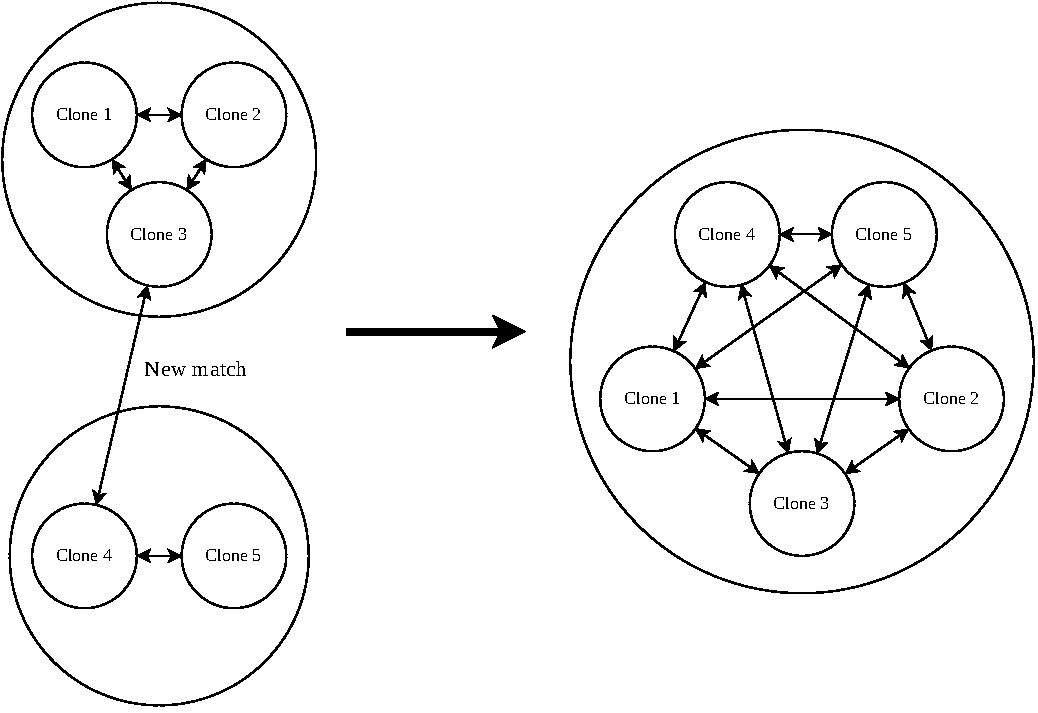
\includegraphics[width=0.95\textwidth]{figures/cloneaggregation.drawio.pdf}
    \end{center}
    \caption{Clone class aggregation when a new match is found}
    \label{fig:cloneaggregation}
\end{figure}

\Todo{Squiggly arrow}


\begin{algorithm}[t]
  \SetAlgoLined\DontPrintSemicolon
    \algo{\GetCloneMap{index, cloneIndices}}{
        $\Var{n} \gets \Access{\Var{cloneIndices}}{\Var{len}}$ \;
        $\Var{cloneMap} \gets \textrm{Empty map with type: } \Var{int} \rightarrow \Var{CodeClone}$ \;\;

        
        \For{$\Var{i} \From 0 \To \Var{n} - 1$}{
            $\Var{firstIndex} \gets \ArrayAccess{\Var{cloneIndices}}{\Var{i}}$ \;
            $\Var{secondIndex} \gets \ArrayAccess{\Var{cloneIndices}}{\Var{i}}$ \;
            $\Var{size} \gets \LCP{\ISA{\Var{firstIndex}}} - 1$ \;\;


            \Comment{Use SourceMap function to get ranges and documents of clones}
            $\Var{firstRange} \gets \textrm{Get source between firstIndex and
            (firstIndex + size)}$ \;
            $\Var{secondRange} \gets \textrm{Get source between secondIndex and
            (secondIndex + size)}$ \;\;

            $\Var{firstDocument} \gets \Access{\Var{firstRange}}{\Var{document}}$ \;
            $\Var{secondDocument} \gets \Access{\Var{secondRange}}{\Var{document}}$ \;\;
            
            \Comment{Build clone objects if they don't exist}
            \If{$\Var{firstIndex} \NotIn \Var{cloneMap}$}{
                $\Var{firstClone} \gets \New
                \CodeClone{$\Access{\Var{firstDocument}}{\Var{URI}},
                \Var{firstRange}$}$ \;
                $\Put{$\Var{cloneMap}, \Var{firstIndex}, \Var{firstClone}$}$ \Comment{Put
                clone with firstIndex as key}
            }
            \If{$\Var{secondIndex} \NotIn \Var{cloneMap}$}{
                $\Var{secondClone} \gets \New
                \CodeClone{$\Access{\Var{secondDocument}}{\Var{URI}},
                \Var{secondRange}$}$ \;
                $\Put{$\Var{cloneMap}, \Var{i}, \Var{secondClone}$}$ \Comment{Put
                clone with secondIndex as key}
            } \;

            \Comment{Union clone classes}
            \UnionCloneClass{\Get{$\Var{cloneMap}, \Var{firstIndex}$}, \Get{$\Var{cloneMap,
            \Var{secondIndex}}$}} \;
        }
        \Return $\Var{cloneMap}$
    }

  \vspace{0.5cm}
  \caption{Build clone-map given the clone indices in the fingerprint}
  \label{alg:buildclonemap}
\end{algorithm}


\chapter{Implementation: Incremental detection}

The following chapter will present the algorithm which efficiently updates the list of
clones, without having to rebuild the different structures from scratch. Given an edit
to a file in the project, we will be able to update the document index, fingerprints,
suffix array and list of clones faster than the initial detection.

An incremental update is run whenever a document is changed. The document index is
signalized of a change either when a file is saved, or on any keystroke. This is
configurable by the client. When the document index is changed, an incremental update of
the clones is run, and the clone-list is updated.

\section{Affordable operations}

Before looking at the approach, it is useful to determine the time cost associated with
different operations. If we can for example afford to iterate over the contents of a
single file, that will be useful for our algorithm. Table \ref{table:affordableoperations}
shows which operations are affordable or not for an incremental update.

\begin{table}[t!]
	\begin{center}
		\begin{tabular}{|p{1in} | p{1in} | p{0.6in} | p{2.5in}|}
			\hline

			Description                    & Complexity              & Affordable & Explanation                               \\\hline

			Content of all files           & $O(|\Var{code\ base}|)$ & No         & Iterating over the
			entire code base will be the same complexity as the initial detection,
			therefore this operation is too slow.                                                                             \\\hline

			Content of a file              & $O(|\Var{file}|)$       & Yes        & Iterating over the content
			of a single file is likely a very small percentage of the entire code
			base.                                                                                                             \\\hline

			Parsing a file                 & $O(|\Var{file}|)$       & No         & While the complexity of
			parsing a single file is still linear in the size of the file, parsing a large
			file from scratch can take a significant amount of time in practice.                                              \\\hline

			Incrementally reparsing a file & $O(|\Var{edit}|)$       & Yes        & Re-using the
			AST of a file in order to speed up the parsing of the same file with
			after an edit is significantly faster than parsing the entire file.                                               \\\hline

			Document index                 & $O(|\Var{documents}|)$  & Yes        & The number of files in a code
			base is likely many orders of magnitude smaller than the size of the code base
			itself.                                                                                                           \\\hline

			Clones                         & $O(|\Var{clones}|)$     & Yes        & The number of clones in the code base and
			the area they cover is likely a very small portion of the code base itself.
			itself.                                                                                                           \\\hline
		\end{tabular}
		\caption{Affordable operations for incremental updates}
		\label{table:affordableoperations}
	\end{center}
\end{table}


\section{Updating the document index}

The first step of an incremental update is to update the document index. We will also look
at how we can reduce memory usage of the index without a loss in terms of the time
complexity of the updates.

As shown in the document interface, each document stores its own content, AST and
fingerprint. It is not strictly necessary to store either the content or the AST in memory
all the time, as it is likely that only a handful of files are open in the IDE at once.
Therefore, in the initial detection, we can free the memory of the file content and AST
for each document after the fingerprint has been computed. However, if a file is opened in
the IDE, the file can now be changed, so we should facilitate efficient updates for these
files only. When a file is opened, the file content should be read from the disk and
updated via the \verb|textDocument/didChange| messages sent from the client. It is also
important to keep the AST of the opened file in memory in order to facilitate incremental
reparsing of the opened files. 

When a file is opened, the LSP client sends a \verb|textDocument/didOpen| message to the
server, which finds the relevant document $D$ in the index, and sets the following fields:

\begin{flalign*}
&\Access{D}{open} = \True \\
&\Access{D}{AST} = \Parse{D} \\
&\Access{D}{content} = \Read{$\Access{D}{uri}$}
\end{flalign*}

After the document fields have been set, the document is ready to receive updates. When
the LSP client sends a \verb|textDocument/didChange| message, the message consists of the
URI of the edited file, the range of the content which has changed, and the content which
has potentially been inserted. This range is then used in a tree-sitter incremental
reparse of the file content. After this reparse, we have efficiently updated a documents
content and AST. After this update, we also set $\Access{D}{changed} = \True$

\section{Updating fingerprints}

With the updated AST for all documents, we can update the fingerprint of all documents
which have been changed. For each document $D$ where $\Access{D}{changed} = \True$, the
fingerprint for D may have changed. Calculating the fingerprint is the same process as in
the initial detection, where we first query the AST for all nodes of a certain type, then
for each matched node $N$, we extract and fingerprint all the tokens which $N$ covers,
using the same fingerprint mapping as was used for the initial detection.

An additional change we have to consider when incrementally updating fingerprints is that
for a document $D$, $\Access{D}{start}$ and $\Access{D}{end}$ which corresponds to the
range which $D$ covers in the fingerprint, may have changed. Also, any document $D_1$
where $\Access{D_1}{start} > \Access{D}{start}$ could also have its range changed. This is
solved while updating each documents fingerprint by counting the number of tokens in each
document after updating, and setting the appropriate \verb|start| and \verb|end| fields.

\Todo{Algorithm for updating document index here}

\Todo{Figure which displays three documents, with old and new fingerprint}

\section{Computing edit operations}

Now that the fingerprint has been updated, we could build the suffix array from scratch
and already see a substantial improvement in performance. The major bottleneck of the initial
detection is to parse and fingerprint the entire code base. However, the updating of the
suffix array can and should also be updated incrementally to further improve efficiency.

The input to the dynamic suffix array algorithm is a set of edit operations. Therefore, we
need to know what exactly has changed in the fingerprint before we can update the suffix
array. We need to determine what edit operations have happened. Edit operations are either
deleting, inserting or substituting a section of the code.

There are two approaches we could take to determine the edit operations. The first is to
look at the ranges that the LSP client sends with each \verb|textDocument/didChange|
message and determine which tokens in the fingerprint have been affected by this message.
However, this approach tightly couples the algorithm to LSP and the scenario where we know
the exact ranges of each change. Also, we might do unnecessary amounts of operations if we
do multiple edits, since some operations could cancel each other out, for example by
inserting and then deleting some text.

The other approach is to determine the changes of the fingerprint via an edit distance
algorithm. An edit distance algorithm is an algorithm which calculates the distance
between two strings $S_1$ and $S_2$. Distance between two strings is the minimum number of
edit operations (insert, delete, substitute) which is required to transform $S_1$ into
$S_2$. Many of the algorithms which calculates the edit distance also allows computing
what the operations are.

The classic algorithm for calculating edit distance operations is attributed to Wagner and
Fischer~\cite{WagnerFischer}. The input to the algorithm is two strings $S_1$ and $S_2$ of
length $n$ and $m$. The output will be the set of operations needed to turn $S_1$ into
$S_2$. This algorithm is based on dynamic programming where a matrix $M$ is filled from
top to bottom and then the operations are inferred from $M$. Algorithm
\ref{alg:wagnerfischerfill} shows how the edit distance matrix is filled and
\ref{tab:wagnerfischermatrix} shows an example matrix.

\begin{figure}[t]
    \begin{center}
	$$
		\sum^{n}_{i = 0}{M[i][0] = i}
	$$
	$$
		\sum^{m}_{j = 0}{M[0][j] = j}
	$$

	\begin{gather*}
		M[i][j] =
		\begin{cases}
			M[i-1][j-1] & \mathrm{if\ } S_1[i] = S_2[j] \\
            1 + \Min{$M[i-1][j-1], M[i][j-1], M[i-1][j-1]$}
		\end{cases}
	\end{gather*}
	\caption{Edit distance recurrence}
	\label{eq:editdistancerecurrence}
    \end{center}
\end{figure}

Each index $i, j$ in $M$ contains the edit distance value between the substrings
$\ArrayAccess{S_1}{0..i}$ and $\ArrayAccess{S_2}{0..j}$ The values in $M$ is calculated by
determining what is the cheapest operation to do at a certain location to make the
substrings equal. This can be determined by looking at the three surrounding indices in
$M$: $\MatrixAccess{M}{i - 1}{j - 1}$, $\MatrixAccess{M}{i - 1}{j}$ and
$\MatrixAccess{M}{i}{j - 1}$. Each of these indices equate to deleting, inserting or
substituting a character in $S_1$. The recurrence in figure
\ref{eq:editdistancerecurrence} describes the algorithm.


\begin{algorithm}[htp]
  \SetAlgoLined\DontPrintSemicolon
    \algo{\WagnerFischerEditDistance{$S_1$, $S_2$}}{
        $\Var{n} \gets \Len{$\Var{S}_1$}$ \;
        $\Var{m} \gets \Len{$\Var{S}_2$}$ \;
        $\Var{matrix} \gets \mathrm{new\ array}[\Var{n} + 1][\Var{m} + 1]$ \;\;


        \For{$i \From 0 \To n$}{
            $\MatrixAccess{\Var{matrix}}{\Var{i}}{0} = \Var{i}$
        } \;

        \For{$i \From 0 \To m$}{
            $\MatrixAccess{\Var{matrix}}{\Var{0}}{i} = \Var{i}$
        } \;

        \For{$i \From 1 \To n$}{
            \For{$j \From 1 \To m$}{
                \If{$\ArrayAccess{\Var{S}_1}{\Var{i} - 1} = \ArrayAccess{\Var{S}_2}{\Var{j} - 1}$}{
                    $\MatrixAccess{\Var{matrix}}{\Var{i}}{\Var{j}}  = \MatrixAccess{\Var{matrix}}{\Var{i - 1}}{\Var{j - 1}} $
                }
                \Else {
                    $\Var{delete} \gets \MatrixAccess{\Var{matrix}}{\Var{i} - 1}{\Var{j}}$ \;

                    $\Var{insert} \gets \MatrixAccess{\Var{matrix}}{\Var{i}}{\Var{j - 1}}$ \;

                    $\Var{substitute} \gets \MatrixAccess{\Var{matrix}}{\Var{i - 1}}{\Var{j - 1}}$ \;\;

                    $\MatrixAccess{\Var{matrix}}{\Var{i}}{\Var{j}}  = \Min{$\Var{insert},
                    \Var{delete}, \Var{substitute}$} + 1$

                }
            }
        }

        \Return $\Var{matrix}$
    }

  \vspace{0.5cm}
  \caption{Fill edit distance matrix using Wagner-Fischer algorithm}
  \label{alg:wagnerfischerfill}
\end{algorithm}

\begin{table}
	\begin{center}
		\begin{tabular}[c]{c|c|c|c|c|c|c|c|c|c|}
			  &                      & D                    & E                    & M                    & O                    & C                    & R                    & A                    & T                    \\\hline
			  & \cellcolor{blue!25}0 & 1                    & 2                    & 3                    & 4                    & 5                    & 6                    & 7                    & 8                    \\\hline
			R & 1                    & \cellcolor{blue!25}1 & 2                    & 3                    & 4                    & 5                    & 5                    & 6                    & 7                    \\\hline
			E & 2                    & 2                    & \cellcolor{blue!25}1 & 2                    & 3                    & 4                    & 5                    & 6                    & 7                    \\\hline
			P & 3                    & 3                    & \cellcolor{blue!25}2 & 2                    & 3                    & 4                    & 5                    & 6                    & 7                    \\\hline
			U & 4                    & 4                    & \cellcolor{blue!25}3 & 3                    & 3                    & 4                    & 5                    & 6                    & 7                    \\\hline
			B & 5                    & 5                    & 4                    & \cellcolor{blue!25}4 & 4                    & 4                    & 5                    & 6                    & 7                    \\\hline
			L & 6                    & 6                    & 5                    & 5                    & \cellcolor{blue!25}5 & 5                    & 5                    & 6                    & 7                    \\\hline
			I & 7                    & 7                    & 6                    & 6                    & 6                    & \cellcolor{blue!25}6 & 6                    & 6                    & 7                    \\\hline
			C & 8                    & 8                    & 7                    & 7                    & 7                    & 6                    & \cellcolor{blue!25}7 & 7                    & 7                    \\\hline
			A & 9                    & 9                    & 8                    & 8                    & 8                    & 7                    & 7                    & \cellcolor{blue!25}7 & 8                    \\\hline
			N & 10                   & 10                   & 9                    & 9                    & 9                    & 8                    & 8                    & 8                    & \cellcolor{blue!25}8 \\\hline

			\hline
		\end{tabular}
	\end{center}
	\caption{Edit distance matrix for REPUBLICAN $\rightarrow$ DEMOCRAT}
	\label{tab:wagnerfischermatrix}
\end{table}


The edit operations can then be inferred from $M$ by backtracking from the bottom-right
index, to the top-left, giving us the edit operations in reverse. At each position $i, j$
we choose either of the 3 surrounding indices, the same indices which were used to
determine the value originally. Choosing the left index ($i, j - 1$) equates to inserting
the character $\ArrayAccess{S_2}{j - 1}$ at position $i - 1$. Choosing the top index ($i -
1, j$) equates to deleting the character $\ArrayAccess{S_1}{i - 1}$. Choosing the top-left
index ($i - 1, j - 1$) equates to substituting $\ArrayAccess{S_1}{i - 1}$ with
$\ArrayAccess{S_2}{j - 1}$. If these characters are already equal, the operation can be
ignored. For example in table \ref{tab:wagnerfischermatrix}, the first operation is to
substitute \verb|R| with \verb|D| at position $0$. Afterwards \verb|P| and \verb|U| is
deleted at position $2$. Then the \verb|B| which is now at position $2$ is substituted by
\verb|M|. This continues with more substitutions until we finally have \verb|DEMOCRAT|.

\Todo{Now collect operations together and explain memory issue + Hirschbergs}

In the next phase we will feed the edit operations into an algorithm which dynamically
updates our suffix array based on those operations. However, this algorithm will be more
efficient if the operations are combined to singular inserts, deletes or substitutes of
strings more than one character. The edit distance algorithm outputs only single character
operations, meaning we insert, delete or substitute a single character at a time. We
therefore want a way to combine these operations to ``larger'' operations.

One way to do this is to simply combine operations which are sequenced in the matrix. For
example in...



\section{Dynamic suffix arrays}

\section{Storing old clones}
